\section{Isoperimetric Quotient}\label{sec:isoper}
\zs{\textbf{  I think the same proof actually goes through here. Take a bite from the top and bottom. Since the bites get sent to different size bites, one isn't the rotation/translation of the other, and because they started from the same circle, scaling doesn't fix the problem. The one with the bigger bite taken out has both smaller area and larger perimeter, so its PP is strictly worse.  }}
\zs{The proof here is pretty informal.  I don't know if it's worth doing; the calculus needed is super gross. }

\zs{One way we can include this without having to compute a bunch of path integrals is to move the Polsby-Popper section to after Reock, then this can be rolled into that section as part of the `discussion' or whatever.}

We remarked at the end of Section~\ref{sec:pp} that a more principled version of an isoperimetric quotient may avoid the failure of the ordinary Polsby-Popper score to induce an ordering which can be preserved by some map projection.

\begin{definition}
We define the \textbf{isoperimetric quotient score} of a region $\Omega$ to be$$
\mathrm{IPQ}(\Omega)=
\begin{cases}
\frac{4\pi \ \mathrm{area}(\Omega)}{\mathrm{perim}(\Omega)^2} \text{ in the plane},\\[10pt]
\frac{\mathrm{area}(\Omega)^2 - 4\pi \ \mathrm{area}(\Omega)}{\mathrm{perim}(\Omega)^2}\text{ on the sphere}
\end{cases}
$$
\end{definition}

This score properly resolves the issue of scale-noninvariance, and the isoperimetric quotient scores of circles in the plane \textit{and} caps on the sphere are one, regardless of their size.

We'll prove order non-preservation in the same way as before, and we built all of the machinery needed to do it in the previous section.  Since any order-preserving map projection needs to preserve the maximizers and caps and circles maximize the isoperimetric quotient score, we can restrict our attention to map projections which send caps to circles.  We showed in the previous section that these are exactly the projections which are the composition of the stereographic projection and a scaled isometry of the plane.  Since this score is scale-invariant, it is preserved by scaled isometries, so we only need to demonstrate the existence of regions on the sphere whose scores are permuted by the stereographic projection.


\begin{theorem}
There exist two regions on the sphere $A$ and $B$ such that $\mathrm{IPQ}(A)>\mathrm{IPQ}(B)$ but under the stereographic projection $\varphi$, $\mathrm{IPQ}(\varphi(A)))<\mathrm{IPQ}(\varphi(B))$.
\end{theorem}

\begin{figure}
    \centering
    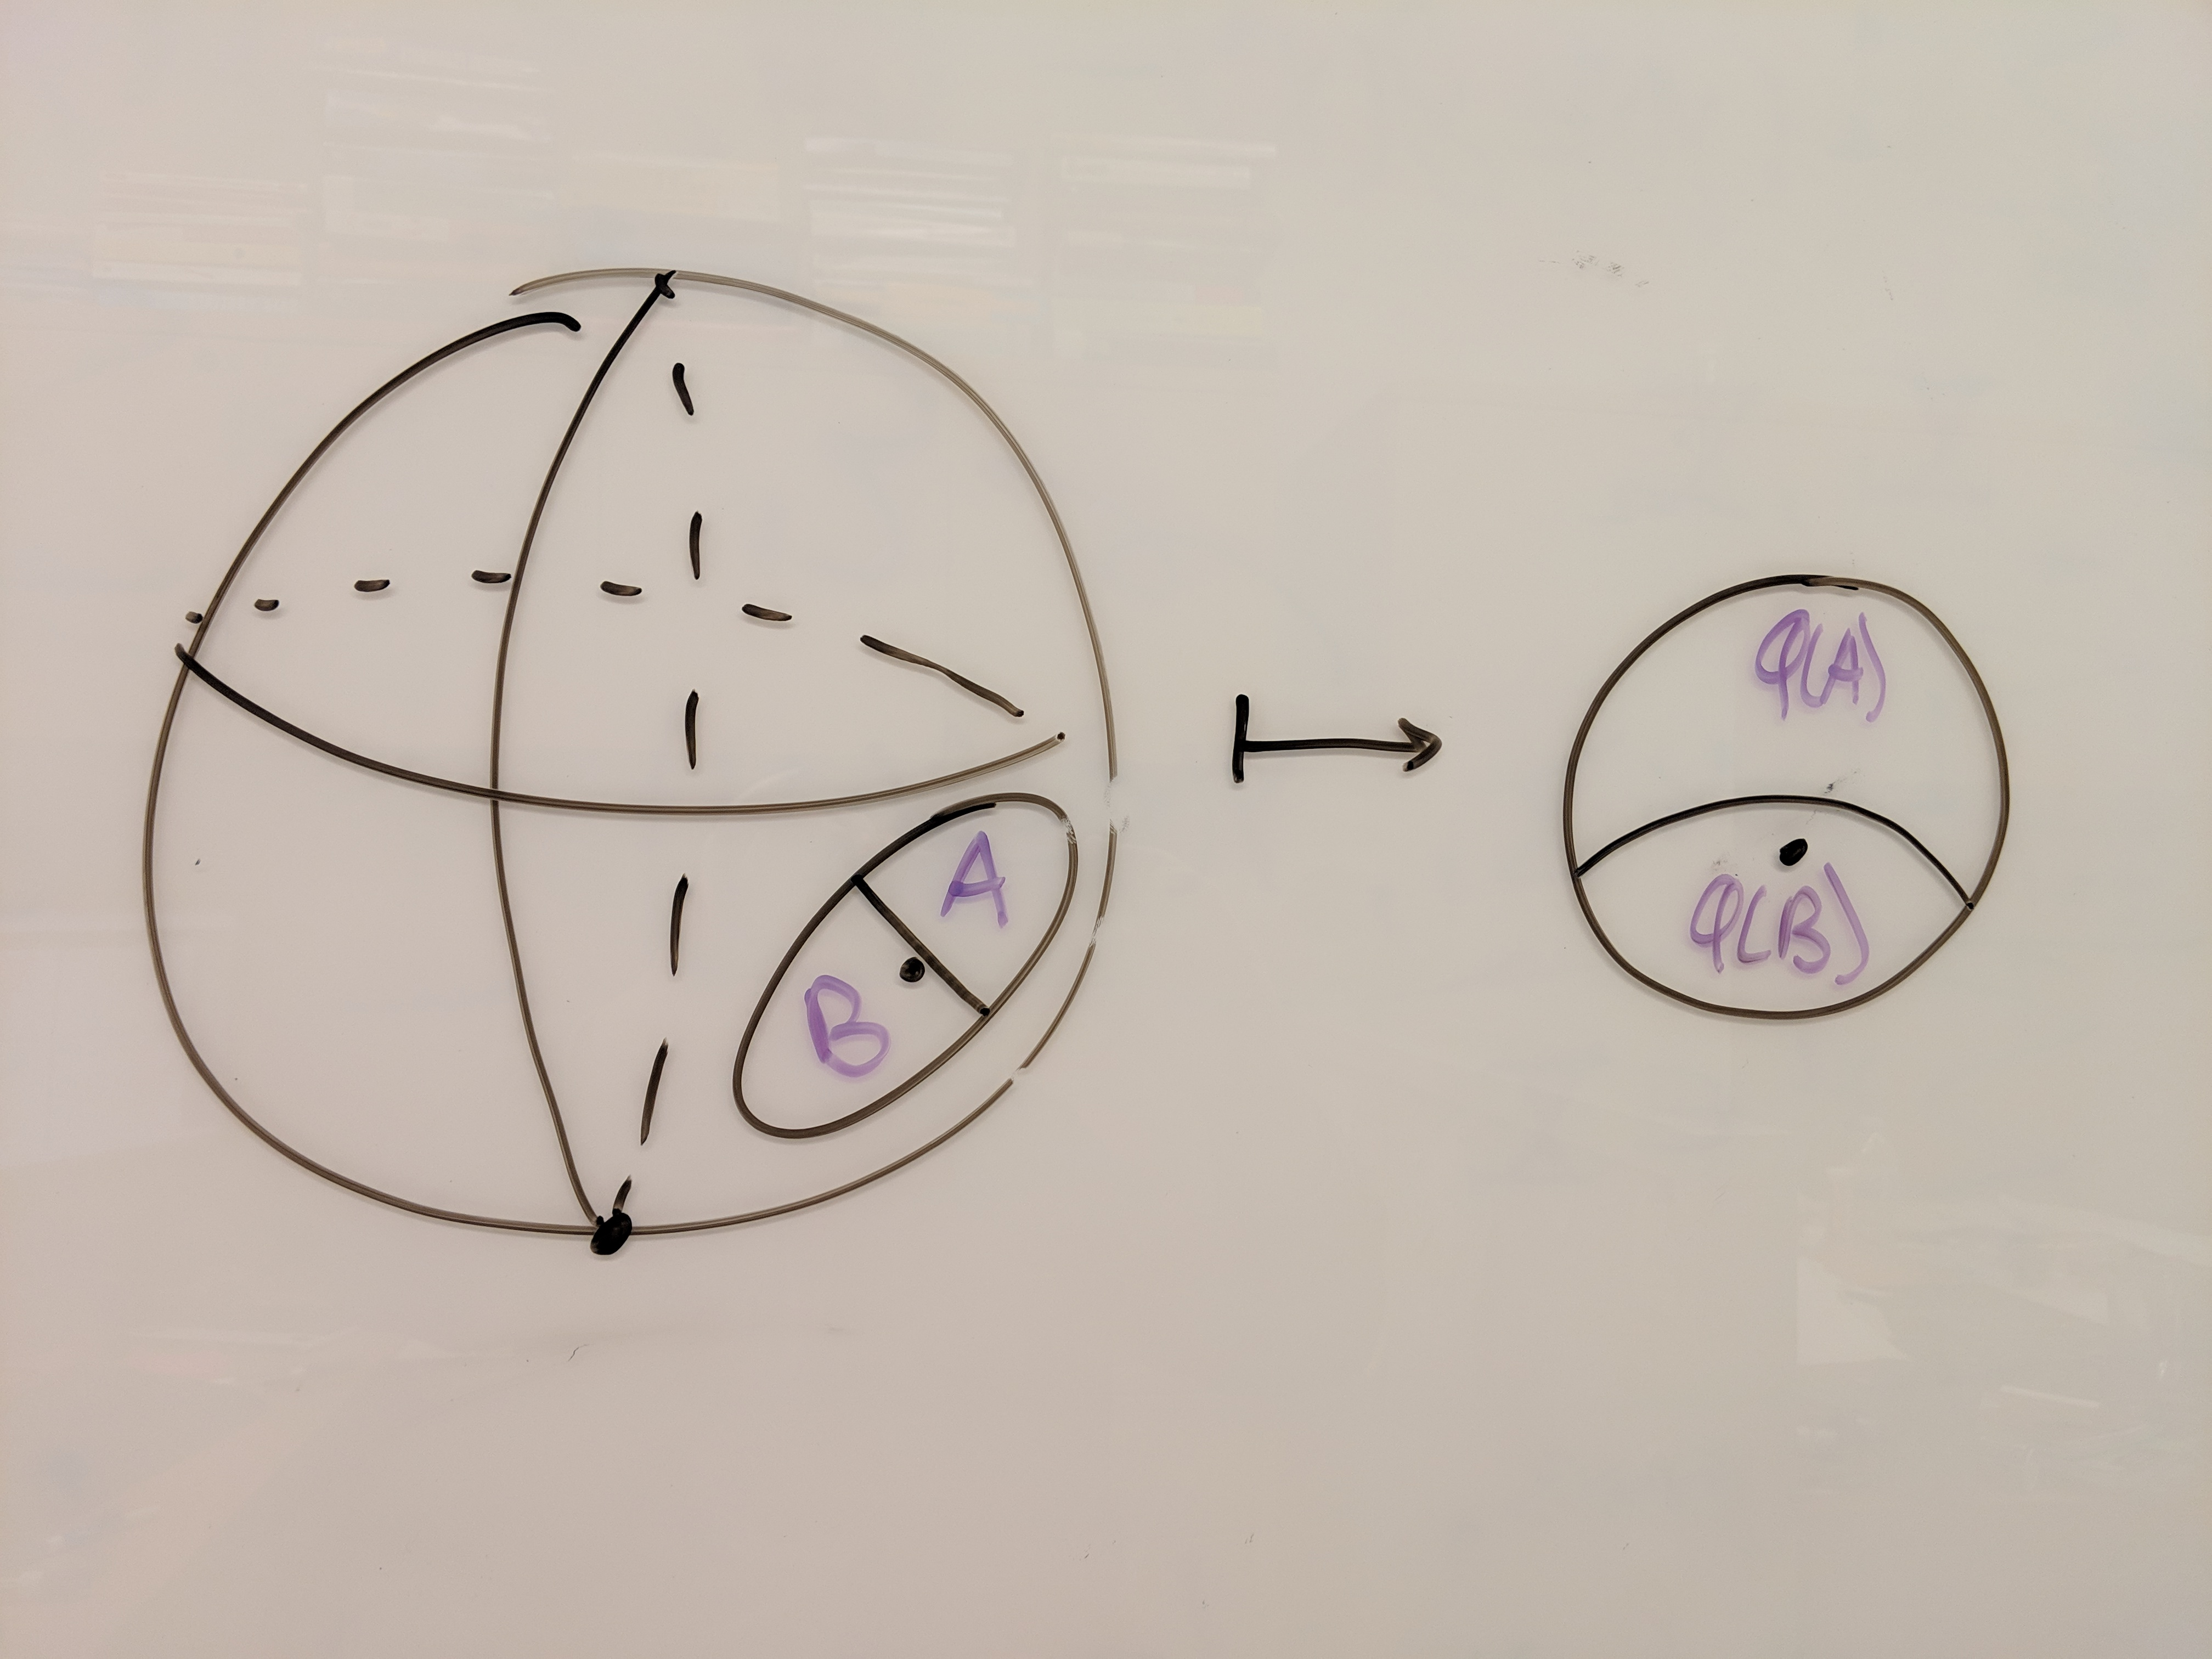
\includegraphics[width=.8\textwidth]{figs/stereo_ipq.jpg}\\
    \caption{ The image of a cap away from the south pole under the stereographic projection. }
    \label{fig:stereoipq}
\end{figure}



\begin{proof}
Let $C$ be a cap with its center slightly away from the south pole, and divide it into a `top' and `bottom' half with the plane that meets the great circle connecting the poles and cap's center orthogonally.  This divides the cap into two pieces with equal area and perimeter, and therefore equal isoperimetric quotient scores.  Shift this division line down so that the top part of the circle has a slightly higher than the bottom.  We let the top part be $A$ and the bottom be $B$.  The stereographic projection sends caps to circles, but does not preserve the \textit{centers} of such caps away from the south pole, and will send the slightly perturbed division line to a nearly circular arc (Figure~\ref{fig:stereoipq}).  

If we had used the original division of the cap into exact halves, then in the plane, the isoperimetric quotient score of $\varphi(A)$ would be strictly less than that of $\varphi(B)$. Since we can choose our perturbation to be small enough to not reverse this order, we have constructed our example of a pair of regions whose isoperimetric score order is not preserved by the stereographic projection.

\end{proof}


The remainder of the argument follows from our previous results.  Lemma~\ref{lem:noafflin} says that no scaled isometry can correct for the permutation of score ordering, so there does not exist a map projection which preserves the ordering over regions induced by the isoperimetric quotient score.






